\section{Validación}

En la presente sección se describirán imágenes del prototipo preparado de la aplicación, estas imágenes se han tomado desde el motor gráfico del juego en su modo de edición. 

\subsection{Prototipo de validación funcional}

\subsubsection{Repositorio}

\url{https://github.com/Hokers/IngSoft_Caso4_Rojas_Romero.git}

\subsubsection{Imagenes}

\begin{figure}[H]
\centerline{
\includegraphics[width=15cm]{imgs/Game_2.PNG}}
\caption{Menu principal aplicación.}
\label{game_2}
\end{figure}

\begin{figure}[H]
\centerline{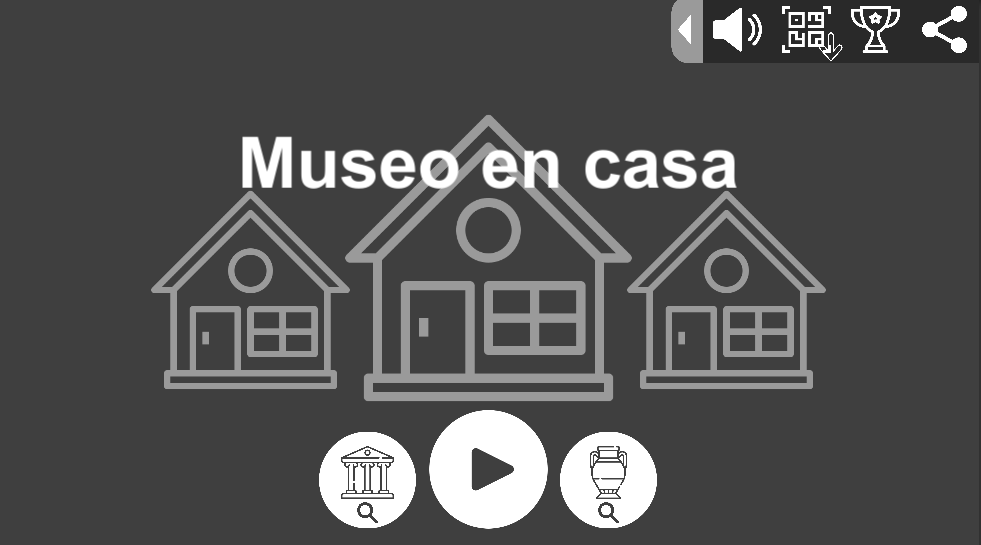
\includegraphics[width=15cm]{imgs/Game_1.PNG}}
\caption{Menu principal aplicación con menu de opciones desplegado.}
\label{game_1}
\end{figure}

\begin{figure}[H]
\centerline{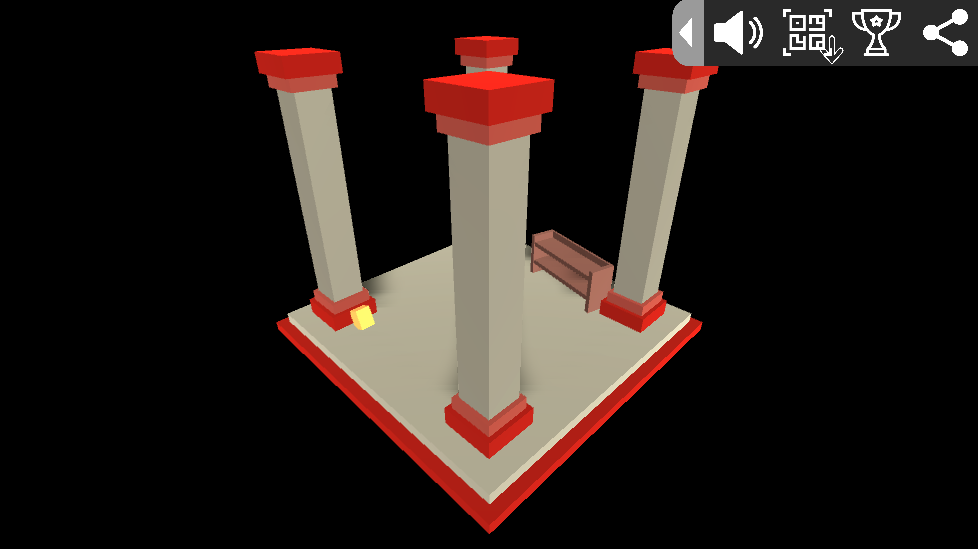
\includegraphics[width=15cm]{imgs/Game_4.PNG}}
\caption{Escena de juego mostrando una habitación del museo.}
\label{game_4}
\end{figure}

\begin{figure}[H]
\centerline{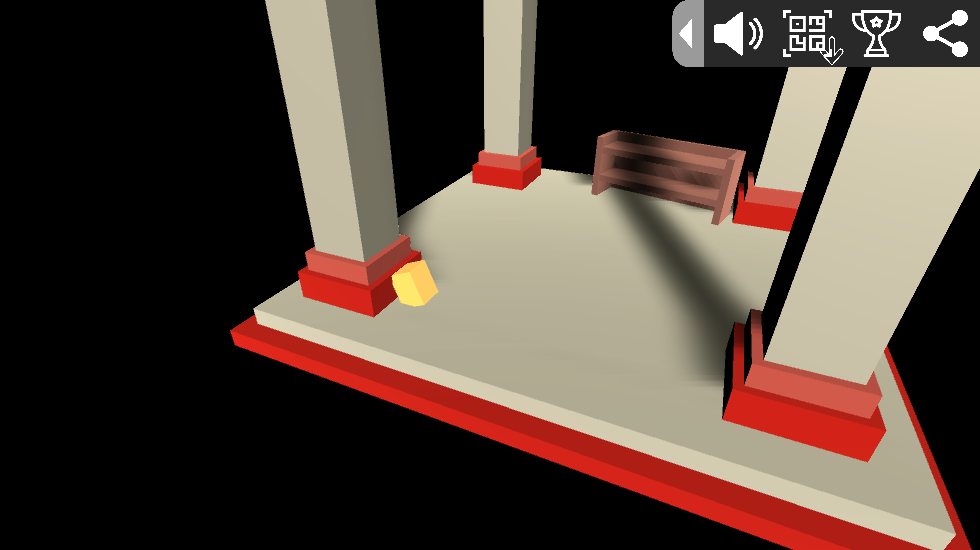
\includegraphics[width=15cm]{imgs/Game_5.PNG}}
\caption{Acercamiento a pieza a descubrir del museo.}
\label{game_5}
\end{figure}

\begin{figure}[H]
\centerline{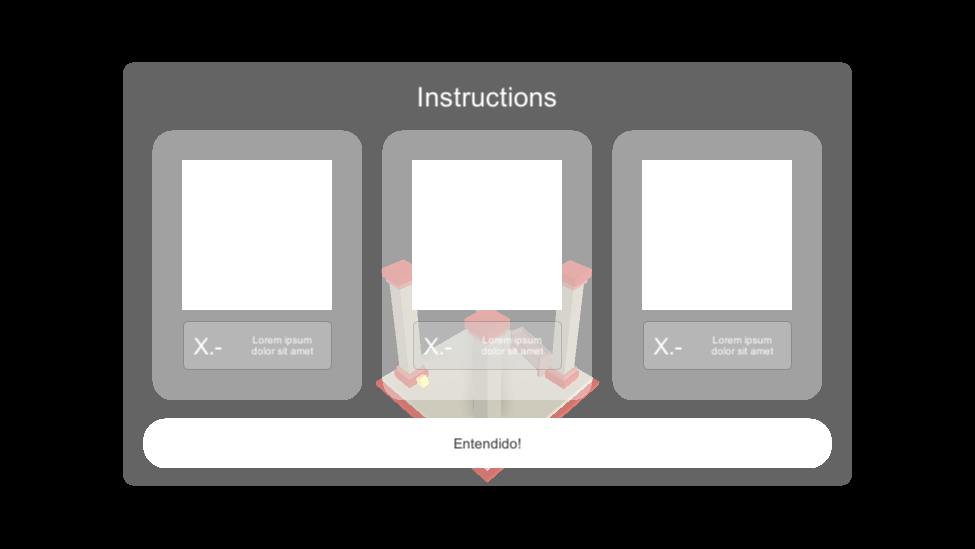
\includegraphics[width=15cm]{imgs/Game_3.PNG}}
\caption{Escena de juego mostrando pantalla de tutorial.}
\label{game_3}
\end{figure}